
%(BEGIN_QUESTION)
% Copyright 2013, Tony R. Kuphaldt, released under the Creative Commons Attribution License (v 1.0)
% This means you may do almost anything with this work of mine, so long as you give me proper credit

In this oily water sump process, two submersible pumps move water out of the sump based on liquid level measurement inside the sump:

$$\includegraphics[width=15.5cm]{i0005rx01.eps}$$

Examine this P\&ID and answer the following questions:

\begin{itemize}
\item{} Why are ``check'' valves installed on the discharge lines of pumps P-407 and P-408?
\vskip 10pt
\item{} Supposing pump P-408 is the only one running, qualitatively determine the effects of pinching off the block valve immediately upstream of pressure gauge PG-419 on the following variables (e.g. {\it increase}, {\it decrease}, or {\it remain the same}):
\itemitem{} Pressure at the pump's discharge port
\itemitem{} Pressure registered by PG-419
\itemitem{} Electrical current to the driving motor
\itemitem{} Flow rate of water through filter S-401
\itemitem{} Pressure registered by PG-419
\itemitem{} Oily water level inside the sump
\end{itemize}

\underbar{file i04794}
%(END_QUESTION)





%(BEGIN_ANSWER)

\begin{itemize}
\item{} Why are ``check'' valves installed on the discharge lines of pumps P-407 and P-408? {\it To prevent oily water from returning to the sump (from which it came) when only one pump is running.}
\vskip 10pt
\item{} Supposing pump P-408 is the only one running, qualitatively determine the effects of pinching off the block valve immediately upstream of pressure gauge PG-419 on the following variables (e.g. {\it increase}, {\it decrease}, or {\it remain the same}):
\itemitem{} Pressure at the pump's discharge port ({\it increase})
\itemitem{} Pressure registered by PG-419 ({\it decrease})
\itemitem{} Electrical current to the driving motor ({\it increase})
\itemitem{} Flow rate of water through filter S-401 ({\it decrease})
\itemitem{} Pressure registered by PG-419 ({\it remain the same})
\itemitem{} Oily water level inside the sump ({\it cannot tell})
\end{itemize}

The last effect (oily water sump level) is unknown because we do not know how the reduced flow of pump P-408 compares to the flow rate of water entering the sump.  If the flow rate of P-408 still exceeds the input flow to the sump, the level will continue to drop although not as fast as before pinching off the block valve.  If the pump's flow rate exactly equals the influent rate, the sump level will remain constant.  If the pump's flow rate has decreased to a point where it is less than the influent flow rate, the sump level will actually rise!

%(END_ANSWER)





%(BEGIN_NOTES)


%INDEX% Process: oily water sump (realistic P&ID shown)

%(END_NOTES)


